\documentclass[a4paper]{report} % estilo do documento

\usepackage[utf8]{inputenc} %encoding do ficheiro
\usepackage[portuges]{babel} % para língua portuguesa
\usepackage{graphicx} % para importar imagens

\begin{document}

\title{Relatório Trabalho Prático LI1}
\author{Grupo 159\\
\\
Gonçalo Faria e Gonçalo Pereira}
\date{\today}

\maketitle

\tableofcontents



%% Introdução
\chapter{Introdução}

  \section{Contextualização}
    \ No âmbito da cadeira de Laboratórios de Informática 1 (1º semestre do 1º ano de MIEI), o método de avaliação escolhido pelos professores foi a realização de um trabalho em grupos de 2, onde o objetivo era programar de raiz o famoso jogo “Micro Machines”, usando a linguagem de programação Haskell.

  \section{Motivação}
    \ O uso num contexto prático dos conhecimentos adquiridos ao longo do nosso percurso académico sempre foi algo que nos fascinou. Compreender as consequências e benefícios do paradigma de programação funcional é algo abstrato e um desafio de compreender, no entanto com a criação de aplicações estes são mais evidentes e permitem-nos assim desenvolver uma intuição de quando este poderá ser aplicado, no futuro na nossa vida profissional.  
  
  \section{Objectivos}
    \ Os objetivos estabelecidos pelo grupo desde o início foram 4:
    \begin{enumerate}
        \item Ter um trabalho final apelativo;
        \item Ter um trabalho final “smov” com o mínimo de bugs possíveis;
        \item Ter o código da programação o mais simples possível, de modo o jogo correr o mais rapidamente possível;
        \item Conseguir realizar as 2 fases do trabalho antes do dia 15 de Dezembro;
    \end{enumerate}

%% Análise de Requisitos e Especificação do Problema
\chapter{Análise de Requisitos}


\section{Fase 1}
\label{sec:analisefase1}

\ { 1ª Fase do trabalho encontra-se subdividida em 3 Tarefas:} 
  \begin{enumerate}
        \item  \ A Tarefa 1 tem como objetivo contruir um mapa para o jogo. 
        \par Onde o mesmo vai seguir um caminho previamente indicado, sendo esse caminho constituído por inúmeros passos, dos quais podemos ter: 
        \par  \ \textbf{Avanca}; \textbf{Sobe}; \textbf{Desce}; \textbf{CurvaEsq}; \textbf{CurvaDir};              
        \par  \ O mapa em si, consiste numa matriz de peças. Todas estas peças têm uma determinada altura e podem ser do tipo: \textbf{lava}; \textbf{recta}; \textbf{rampa}; \textbf{curva}; Sendo que as peças do tipo recta e curva têm um caraterística acrescida, a \textbf{orientação}.
        \par   \ O foco nesta Tarefa seria receber uma lista de peças e conseguir peça a peça criar o mapa.
        
        \item  \ A Tarefa 2 tem como objetivo verificar se um dado mapa é válido ou não, de acordo com um conjunto de regras inicialmente estabelecidas. 
        \par \ \ \ REGRAS TAREFA 2:
            \begin{itemize}
                \item \small{Existe apenas um percurso e todas as peças fora desse percurso são do tipo lava;}
                \item  \small{O percurso deve corresponder a uma trajetória, tal que começando na peça de partida com a orientação inicial volta-se a chegar à peça de partida com a orientação inicial;}
                \item \small{A orientação inicial tem que ser compatível com a peça de partida. Como é sugerido na imagem abaixo, considera-se que a orientação é compatível com a peça se for possível entrar na peça seguindo essa orientação (note que esta questão só é relevante para as peças do tipo curva e rampa;}
                \item  \small{As peças do percurso só podem estar ligadas a peças do percurso com alturas compatíveis;} 
                \item  \small{Todas as peças do tipo lava estão à altura 0;}
                \item  \small{O mapa é sempre retangular e rodeado por lava, ou seja, a primeira e última linha, assim como a primeira e última coluna são constituídas por peças necessariamente do tipo lava.}
            \end{itemize}
            
        \item \ O objetivo da Tarefa 3 é começar implementação da mecânica do jogo, mais propriamente as movimentações do carro e as suas consequentes interações com o mapa.
        \par  \ Para tal começamos por criar e modelar um Carro, caraterizado por três pontos: \textbf{Posição}; \textbf{Direção}; \textbf{Velocidade};
        \par  \ De seguida tivemos que, dado um estado inicial do carro, calcular o seu estado final após um determinado período de tempo. 

    \end{enumerate}

\section{Fase 2}
\label{sec:analisefasee}

\  { A 2ª Fase do trabalho encontra-se subdividida também ela em 3 Tarefas: }

        \begin{enumerate}
            \item O objetivo da Tarefa 4 é a partir de ações efetuadas por um jogador num período de tempo atualizar o estado do jogo . 
            \par Para isso é necessário representar o \textbf{Jogo} (o estado interno do jogo) que deverá ser atualizado em cada instante e a \textbf{Ação} algo que vai indicar, por exemplo, se o carro está a acelerar, travar, ou curvar.
            \par O foco desta tarefa é garantir que o estado do jogo atualiza a cada momento corretamente, tendo em conta todas as possibilidades.
            \item O objetivo desta Tarefa ao contrário das outras não é específico para todos os grupos, trata-se de uma Tarefa livre. 
            \par Na Tarefa 5 é pedido que cada grupo implemente todo o jogo usando a biblioteca Gloss. 
            \par A ferramenta Gloss irá tratar de construir a parte gráfica do jogo. Onde cada grupo tem a liberdade de desenhar o jogo à sua maneira.
            \par O foco principal na Tarefa 5 é criar o máximo de elementos gráficos apelativos e criativos, sem nunca perder o foco do jogo, uma corrida de carros.
            \item O objetivo da Tarefa 6 é implementar um bot que jogue o Micro Machines automaticamente. 
            \par Um bot que percorra o percurso da maneira mais eficiente possível, tendo em conta o que o rodeia. A estratégia de jogo a implementar fica ao critério de cada grupo, sendo que a avaliação automática será efetuada colocando o bot implementado a combater com diferentes bots de variados graus de “inteligência”. 
        \end{enumerate}


%% Descrição da Solução Desenvolvida


\chapter{A Nossa Solução}
\label{sec:solucao}

       \ \textbf{ { \LARGE Fase 1} }
       \vspace{5mm}
   
           \section{Tarefa 1}
         
           \vspace{5mm} 
           \par \textbf{Foco Principal:}
           \par \ \  Embora os docentes estejam a incutir nos alunos que esta tarefa deve ser resolvida usando listas de listas existem alternativas bem mais eficientes e acima de tudo mais rápidas e fáceis de a programar. 
           \vspace{4.5mm} 
           \par \textbf{Desenvolvimento:}
           \par \ \ \textbf{ Inspiração} 
           \par \ \ \ \ Embora na linguagem  C existam matrizes, estas não são implementadas pelo compilador nesse formato. De forma a obter maior eficiência o compilador memoriza apenas o endereço do primeiro elemento e a dimensão desejada da matriz final. Isto é genial, pois, assim conseguem-se obter os benefícios adjacentes à manipulação de arrays com a simplicidade de gestão de dados das matrizes. 
           \vspace{1.7mm} 
           \par \ \ \textbf{ Haskell} 
           \par \ \ \ \ \ Embora, Haskell não apoie arrays (com o Prelude ) podemos usar este método para evitar o uso de listas de listas no processamento dos exercícios pois não só seria custoso no domínio da análise de complexidade do programa como cansativo para o programador. 
           \par \ \ \ \ \ A solução? Criar um tipo de Dados chamado ‘Bidimentional list’ que será composto por um tuplo de inteiros, designado dimensão e também uma lista. 
                    \begin{verbatim}
     data Bidimlist = Bid Dimensao [Peca]
                    \end{verbatim}
           \par \ \ \ \ \ A lista terá sempre, sendo a sua dimensão (x,y),  x y elementos. Ou seja embora não estejamos a usar uma lista de listas a informação desta será guardada na íntegra ( x y é o numero de elementos de uma matriz x por y). 
           \par \ \ \ \ \ \textbf{A posição (i,j) da lista de listas será indexada no elemento  ( j  x ) + i .}
           \par \ \ \ \ \ \textbg{Com estes elementos básico apresentados é agora possível estimar qual será então a solução proposta à tarefa .}
           \par \ \ \ \ \ Iniciar-se-á com a obtenção das dimensões iniciais do tabuleiro e do ponto de partida do caminho, usando as funções auxiliares dos docentes. A orientação inicial será, por convenção \textbf{Este} e a \textbf{Altura 0}.
           \par Tendo como argumentos a ORIENTAÇÃO o PASSO e a ALTURA . Podemos obter qual é a peça que permitirá satisfazer estas condições.
           \par Concorrentemente é também possível saber qual será a próxima posição. Pois é suficiente a orientação e a posição inicial . Todo este processo será recursivamente repetido para os restantes passos do caminho obtendo as sucessivas peças e posições.
           \par 
           \vspace{1.7mm} 
           \par \ \ \textbf{ Processamento } 
           \par \ \ \ \ \ Tendo obtido apenas uma lista de Peças, à priori,  muito inferior ao número de elementos do tabuleiro. 
           \par \ \ \ \ \ Como poderemos satisfazer os requisitos desta Tarefa?
           \vspace{1.7mm} 
           \par \ \ \textbf{  Preencher a lista bidimensional } 
           \par \ \ \ \ \ Com a fórmula mostrada anteriormente temos um método ideal de traduzir as coordenadas das posições em índices na lista bidimensional. 
           \par \ \ \ \ \ Os restantes índices, que um leitor mais precipitado rapidamente denunciaria, serão trivialmente preenchido com a peça lava. 
           \vspace{1.7mm} 
           \par \ \ \textbf{  Detalhes de implementação } 
           \par \ \ \ \ \ De forma a diminuir o tempo de execução significativamente antes de preencher a lista bidimensional peças com a respetiva posição serão agregadas numa lista do duplo (Int , Peça) onde o inteiro é já a tradução das coordenadas da posição. Seguidamente, ocorrerá a ordenação desta lista de duplos em função desses Inteiros. 
           \vspace{1.7mm}  
           \par \ \ \textbf{ Ordenação } 
           \par \ \ \ \ \ Foi usado o célebre algoritmo Quick Sort. Escolhido trivialmente pelo facto de já o ter implementado em haskell ao fazer um dos exercícios das 50 questões. 
           \par \ \ \ \ \ Não se encontra devidamente implementado pois o pivot será sempre o primeiro elemento da lista de cada recursão deste algoritmo. 
           \par \ \ \ \ \ Chegamos a esta conclusão pois existe a possibilidade do primeiro elemento ser ou o maior elemento da lista ou o menor (aproximadamente uma probabilidade de \textbf{(1/2) elevado a (n-2)} disto acontecer para uma lista de tamanho n ), elementos estes que não assegurarão que a lista será devidamente separada (dividida a meio). 
           \vspace{4.5mm}  
           \par \textbf{ Ponto Final: } 
           \par \ \ \ \ \ Após obtida a lista bidimensional ter-se-á unicamente de a converter em lista de lista nas dimensões em que foi originalmente declarada. 
           \par \ \ \ \ \ Isto faz-se segmentando a lista em y sub listas de tamanho x. 
         \vspace{19mm}
           
            \section{Tarefa 2}
           
            \vspace{5mm} 
           \par \textbf{ Foco Principal:} 
           \par \ \ \ \ No todo que é o código da Tarefa 2, a função principal, ‘valida’, recebe um Mapa ao qual vai atribuir um valor Bool que será “True” caso o mapa seja válido ou “False” quando é inválido.
           \vspace{1mm}
                            \begin{verbatim}
 valida :: Mapa -> Bool
                            \end{verbatim} 
                            
           \par \textbf{ Desenvolvimento:} 
           \par \ \ \ \ De maneira a determinar a veracidade do Mapa, tivemos que inicialmente estudar quais os casos que tornariam um mapa inválido, sendo eles:
             \begin{itemize}
                \item \textbf{Mapa Rodeado por lava:}
                \par \ Para o mapa ser válido o mesmo tem de ser rodeado por lava em todos os seus cantos. 
                \par \ Sendo assim tivemos de criar uma função que verifica-se se a primeira e última coluna e a primeira e última linha eram constituídas necessariamente por uma peça do tipo lava.
                \item \textbf{Mapa Retagular:}
                \par \ O mapa é válido se e só se for retangular. Para confirmarmos se um mapa é retangular ou não, criámos uma função que recebe um Bidimlist e que lhe atribui um valor Bool. 
                \par \ Será True toda a vez que o produto de x e y da Bidimlist for igual ao comprimento da lista da mesma.
                \item \textbf{Sequência lógica das Peças:}
                \par \ Como é óbvio o fator mais importante e mais detalhado da Tarefa 2 é a interação de um determinada peça com as suas peças adjacentes. 
                \par \ Para deduzir as consequências de cada interação tivemos de em cada caso particular indicar a sua respetiva consequência. 
                \par \ Temos este exemplo simples, em que as duas peças adjacentes são \textbf{Peca Recta 0} e \textbf{Peca Recta 1}, apesar de serem ambas peças reta como a altura de ambas é diferente o carro nunca poderá passar da primeira peça para a segunda, respetivamente. 
                \par \ Identificada cada uma das possíveis interações, o passo seguinte foi criar uma função que fosse ler as peças da lista que constitui o mapa, peça a peça, e verificar se em cada caso a relação e interação entre elas era válida.
                \item \textbf{Início e fim do Mapa:}
                \par \ Um detalhe muito importante, também a ter em conta é o facto de o mapa ter de iniciar e acabar na mesma peça. Existindo um único caminho possível a percorrer pelo carro a fim de completar o mapa, cruzando a meta.
                \end{itemize}
            \par \textbf{ Ponto Final:} 
            \par \ \ \ \  Com todos estes casos considerados e com o código bem estruturado e válido, a nossa função ‘valida’ será capaz de receber qualquer tipo de Mapa, lê-lo e no final atribuir-lhe um valor de válido ou inválido.    
           \vspace{6mm}
           
           \section{Tarefa 3}
           
           \vspace{5mm} 
           \par \textbf{ Foco Principal:} 
           \par \ \ \ \  O objetivo principal na Tarefa 3 é implementar a função movimenta. Que irá devolver um valor Maybe carro, onde o maybe depende se o carro é destruído ou não.
                            \begin{verbatim}
    movimenta :: Tabuleiro -> Tempo -> Carro -> Maybe Carro 
                            \end{verbatim} 
           \par \textbf{ Desenvolvimento:} 
           \par \ \ \ \ Esta tarefa foi resolvida tentando dividir o problema de movimentar o carro por várias peças, em calcular o movimento do carro em múltiplas etapas. 
           \par \ \ \ \ A função que criámos para processar cada um dos movimentos foi a \textbf{Branch}.
                            \begin{verbatim}
    branch :: Bidimlist -> Carro -> Tempo -> Posicao -> Maybe Carro  
                            \end{verbatim}
           \par \ \ \ \ Isto acontece, pois, nós consideramos que a melhor solução seria aquela em que se dividia o problema de movimentar o carro por 3 pecas por partes.  
           \par \ \ \ \ Designámos por limite a extremidade de uma peça qualquer, ou seja, as paredes laterais, superiores e até mesmo a parede diagonal no caso das curvas. 
           \par \ \ \ \ Um dos nossos problemas nesta tarefa foi determinar o tempo que o carro demorava a atingir um limite. Portanto criámos a função \textbf{intersecT} que se limita a encontrar o tempo de interseção do carro com uma das quatro arestas.
                            \begin{verbatim}
    intersecT :: Velocidade -> Ponto -> (Int,Int) -> Tempo                           
                            \end{verbatim}
            \par \ \ \ \ Uma situação específica é a qual em que o carro irá colidir com uma das duas possíveis diagonais de uma peça Curva.
            \par \ \ \ \ Para calcularmos o tempo que o carro demora até interagir com uma dessas diagonais criámos a função \textbf{insecT}.
                            \begin{verbatim}
    insecT :: Velocidade -> Ponto -> (Int,Int) -> Tempo                            
                            \end{verbatim}
            \par \ \ \ \  Um ponto importantíssimo é o facto da peça em que o carro se encontra ser fundamental, pois determina as diferentes funções que são executadas, visto que diferentes peças têm diferentes limites.
            \par \ \ \ \ Após executada a função que irá processar movimentos na peça específica, vamos começar por ponderar a interseção do carro com todos os limites dessa peça e determinar se algum desses é possível.  
            \par \ \ \ \ Caso não seja possível a interseção do carro com um limite então esse carro vai movimentar-se livremente durante o instante indicado pois sabemos que não ocorreram adversidades.   Caso contrário é calculado o movimento até esse limite e processada uma reação.
            \par \ \ \ \ Os processamentos da reação no caso de colisão têm em conta que o ângulo refletivo é igual ao ângulo incidente e por isso procede à atualização da velocidade.
            \par \ \ \ \ Uma função muito importante é a \textbf{collision}, que visa calcular o vetor velocidade após uma colisão.
                                \begin{verbatim}
    collision :: Velocidade -> (Int,Int) -> Velocidade                               
                                \end{verbatim}
            \par \ \ \ \ Na eventualidade desse limite levar a uma outra peça onde é permissível a movimentação do carro, então o processo é repetido recursivamente até que o carro se destrua ou o tempo acabe. 
            \vspace{5mm}
            \par \textbf{ Ponto Final:} 
            \par \ \ \ \ Temos então uma função que é capaz de calcular qualquer interceção entre o carro e o mapa. Tendo em conta que o estado final do carro após o movimento também é estudado, podendo ele acabar inteirou ou destruído. 
                    
           \vspace{10mm}
           
          \ \textbf{ { \LARGE Fase 2} }
          \vspace{5mm} 
          
          \section{Tarefa 4}
         
           \vspace{5mm} 
           \par \textbf{ Foco Principal:} 
           \par \ \ \ \ Criar uma função que tendo o estado atual do jogo, ao receber uma ação e um determinado período de tempo consiga atualizar o estado do jogo. 
           \vspace{5mm}
           \par \textbf{ Desenvolvimento:} 
           \par \ \ \ \ A função principal desta tarefa é a \textbf{atualiza}, usada para atualizar o estado do jogo dadas as ações de um jogador num determinado período de tempo.
                                \begin{verbatim}
    atualiza :: Tempo -> Jogo -> Int -> Acao  -> Jogo                                
                                \end{verbatim}
           \par \ \ \ \ Para proceder à atualização da velocidade temos que usar a formula genérica \textbf{V = t*a + Vo}
           \par \ \ \ \ Tivemos então que identificar a aceleração a que o carro se encontrava exposto e para isso tivemos de separadamente calcular os diferentes vetores aceleração.
           \par \ \ \ \ Temos então o atrito lateral dos pneus, o atrito normal, a aceleração gravítica e a aceleração do motor.
           \par \ \ \ \ Para calcular estas acelerações usámos as funções: \textbf{acgravitica}; \textbf{acPneus}; \textbf{acAcel}; 
           \par \ \ \ \ Para tal criámos a \textbf{acAtrito} que executa as computações correspondentes ao cálculo da aceleração do atrito no carro.
                            \begin{verbatim}
    acAtrito :: Double -> Velocidade -> (Double , Double)                            
                            \end{verbatim}
            \par \ \ \ \ Seguidamente somámos todos esses vetores da aceleração obtendo assim a aceleração total do carro. 
            \par \ \ \ \ Sucedeu-se então à multiplicação do vetor aceleração total pelo tempo a que o carro estaria exposto à mesma.  Por fim somámos à velocidade inicial do carro. 
            \par \ \ \ \ Uma das funções mais fundamentais desta Tarefa é a \textbf{newvelocity}, pois é nela que a grande maioria das velocidades são calculadas.  
                            \begin{verbatim}
    new_velocity :: Acao-> Propriedades ->Carro -> Tempo
    ->Maybe Orientacao -> Angulo ->Velocidade
                            \end{verbatim}        
            \par \ \ \ \ Um ponto muito importante foi criar uma função que atualizasse o tempo de uso de nitro por parte de cada jogador. Criámos então a função \textbf{updateNitro}, que retribui o Jogo.     
                            \begin{verbatim}
    updateNitro :: Acao -> Tempo -> Jogo -> Int ->Jogo                            
                            \end{verbatim}
            \par \ \ \ \  Finalmente deu-se a atualização do histórico, onde verificamos se a posição atual do carro é diferente da posição à cabeça do histórico, caso seja verdade esta nova posição é adicionada à lista, caso não seja o histórico não ó alterado.
            \par \ \ \ \  Para tal criámos a função \textbf{updateHist}.
                            \begin{verbatim}
    updateHist :: Jogo -> Int -> Jogo                            
                            \end{verbatim}  
           \vspace{5mm}
           \par \textbf{ Ponto Final:} 
           \par \ \ \ \ Para que seja possível que as mecânicas do jogo sejam de alguma forma realistas é crucial que esta componente da aplicação esteja extremamente bem definida e por essa razão nós dedicamos bastante tempo a obter as fórmulas das diferentes acelerações.
           
           \vspace{10mm}
           
           \section{Tarefa 5}
        
           \vspace{5mm} 
           \par \textbf{ Foco Principal:} 
           \par \ \ \ \ Criar um jogo visualmente apelativo, simples de manobrar e o mais completo e divertido possível.
           \vspace{5mm}
           \par \textbf{Desenvolvimento:}
           \par \ \ \ \  Inicialmente antes de nos focarmos em tratar de criar imagens apelativas, colocámos como nossa prioridade tratar de escrever o código na sua totalidade usando a ferramenta \textbf{“Gloss”} de modo a termos em primeira mão o nosso jogo a funcionar e a aparecer perante a nossa tela.  
           \par \ \ \ \ Como qualquer jogo teríamos de criar pelos menos 4 scenes,\textbf{Introdução do Jogo}, \textbf{Menu Inicial}, \textbf{Desenvolvimento do Jogo}, \textbf{Final do Jogo}. Acabámos no entanto por criar 5, acrescentando a possibilidade  de poder escolher em que mapa pretende jogar.
           \par \ \ \ \ Toda a Interface do jogo será controlada usando as \textbf{setas do Keyboard} e a tecla \textbf{“Enter”}.
           \par \ \ \ \ No menu Inicial, temos o logotipo do jogo e de seguida surge um botão \textbf{“Start”} que permitirá dar início ao jogo.
           \par \ \ \ \ Passamos então para a janela que permitirá ao jogador escolher entre 2 mapas. Escolhemos dois mapas, sendo um básico e um bem mais avançado.
           \par \ \ \ \ Chegamos então à quarta tela, a mais detalhada e mais importante, o decorrer do jogo. 
           \par \ \ \ \ Nela podemos identificar: O \textbf{mapa previamente escolhido}, como plano de fundo; As \textbf{4 naves espaciais}, que irão competir entre si; \textbf{4 capacetes} ao qual corresponde uma \textbf{botija de Nitro}. É de referir que \textbf{qualquer capacete ficará cinzento caso a respetiva nave recebe uma penalização}. Já \textbf{a botija ficará cinzenta caso o respetivo veículo gaste todo o seu nitro}.
           \par \ \ \ \ Para além de todos estas funcionalidades introduzimos também a \textbf{animação do nitro} que ocorre logicamente quando o nitro é ativado e também uma mecânica que dá a ilusão ao jogador que o seu carro está a ser seguido com uma câmara, pois colocamos o carro deste ampliado no centro do ecrã. 
           \par \ \ \ \ Por fim quando uma das 4 naves conclui a pista, a quarta tela surge. 	
           \par \ \ \ \ A mesma encontra-se divida em duas possibilidades, onde a escolha de qual delas surge depende do resultado do jogador.
           \par \ \ \ \ Se o mesmo ganhou a corrida irá aparecer \textbf{“You Win”} na tela, caso contrário irá aparecer \textbf{“You Lose”}.
           \par \ \ \ \ No final da corrida o processo repete-se. 
           \vspace{16mm}
           \par \textbf{Ponto Final:}
           \par \ \ \ \ Com todos os nossos objetivos bem executados, logicamente o nosso jogo acabaria por ser apelativo e garantir ao jogador/jogadores um bom entretenimento. Tivemos, no entanto, a desilusão de não conseguir implementar o modo “Multiplayer”,
           
               \begin{figure}[h!]
               \centering
               
\includegraphics [scale = 0.3] {sc1.png}
               \caption{1ª Tela}
               \end{figure}
           
           \begin{figure}[h!]
               \centering
               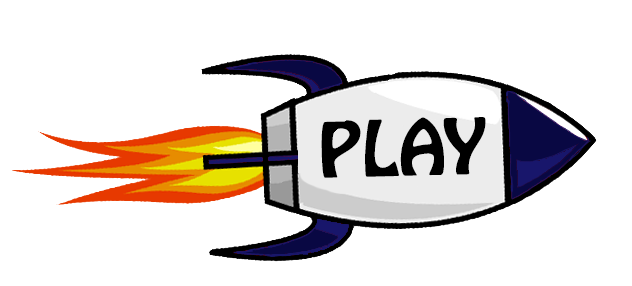
\includegraphics [scale = 0.3] {sc2.png}
               \caption{2ª Tela}
               \end{figure}
           
           \begin{figure}[h!]
               \centering
               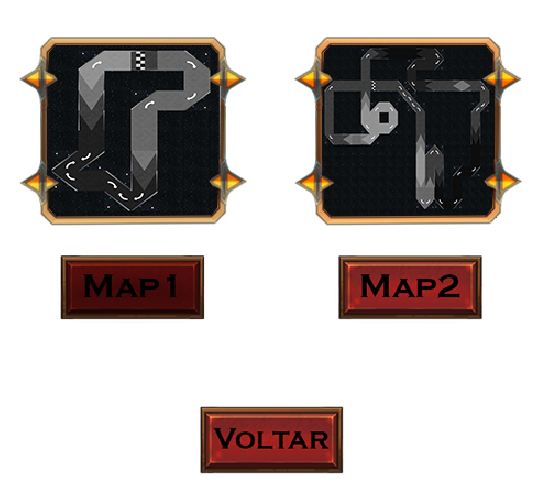
\includegraphics [scale = 0.4] {sc3.png}
               \caption{3ªTela}
               \end{figure}
           
           \begin{figure}[h!]
               \centering
               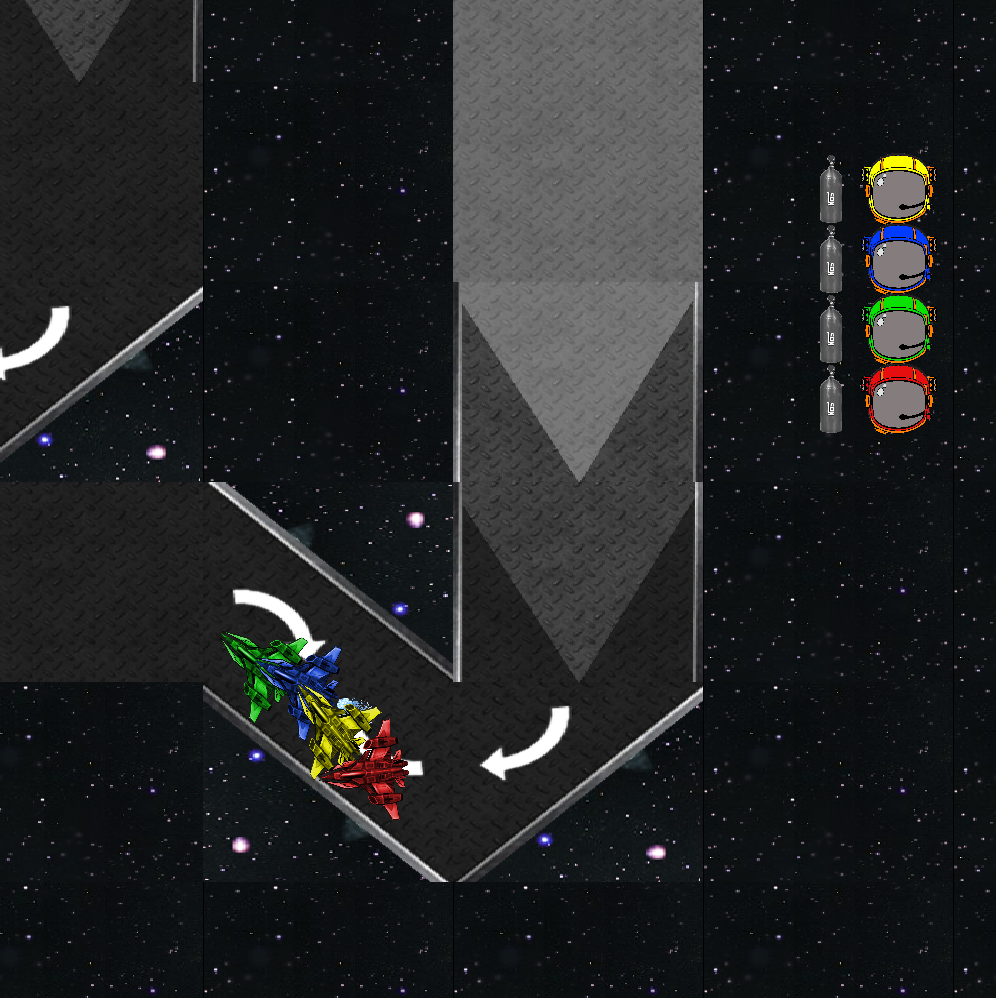
\includegraphics [scale = 0.15] {sc7.png}
               \caption{Possível 4ª Tela}
               \end{figure}
           
           
           \begin{figure}[h!]
               \centering
               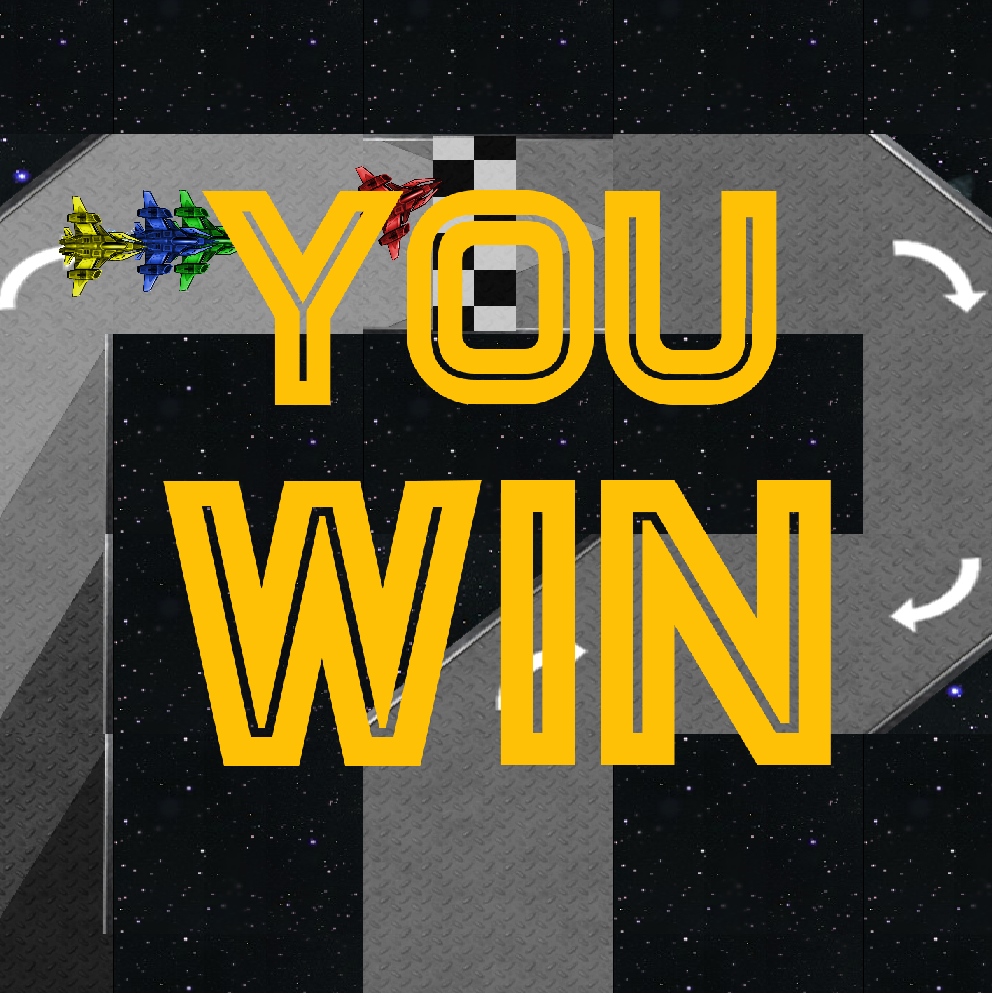
\includegraphics [scale = 0.15] {sc4.png}
               \caption{Possível 5ªTela}
           \end{figure}
           
    
           \section{Tarefa 6}
           
           
           \vspace{5mm} 
           \par \textbf{ Foco Principal:} 
           \par \ \ \ \ O Foco principal desta Tarefa foi criar um bot que conseguisse ler cada situação específica em que o carro se encontrasse em qualquer ponto de um determinado mapa, de modo a rapidamente e facilmente deduzir qual a melhor ação que deve tomar de modo a percorrer o mapa o mais rapidamente possível. 
           \vspace{5mm}
           \par \textbf{Desenvolvimento:}
           \par \ \ \ \ A ação dada pela função \textbf{bot} serão o resultado da mistura de 2 mecanismos diferentes para o cálculo de decisões.
           \par \ \ \ \ Estes mecanismos podem ser vistos como bots independentes,
pois cada um irá produzir para qualquer estado de jogo uma ação, que podia por si só ser a solução a este problema. 
           \par \ \ \ \ No entanto, vários testes intuíram que a junção dos dois bots aumenta significativamente a performance do que ambos individualmente.
           \par \ \ \ \ O primeiro bot designamos por \textbf{conservador}, pois ele foi criado pela necessidade de cumprir as diferentes regras criadas pelos professores (Não passar peças à frente, por exemplo).
           \par \ \ \ \ No entanto este bot é regra geral extremamente lento, pois o seu objetivo é apenas percorrer a peça em que se encontra.
           \par \ \ \ \ O segundo bot a que designamos \textbf{guloso}, usando sensores, tenta determinar qual é a direção que o permitirá evitar limites de forma a conseguir maximizar a velocidade. 
           \par \ \ \ \ O grande problema deste bot, e a principal razão pela qual não foi selecionado como única solução, foi que muitas vezes 'cortava-caminho' (não percorria todas as peças).
           \par \ \ \ \ Isto não era problema para mapas mais restritos, no entanto para mapas mais complexos o bot chegava a evitar secções inteiras.
           \par \ \ \ \ Esta ultima parte só foi problemática porque os professores nos torneios entre os diferentes alunos não permitiam que isto acontece-se.
           \par \ \ \ \ As heurísticas para determinar qual dos dois usar foram bastante simples.
           \par \ \ \ \ Era inicialmente determinando qual extremidade da peça de onde o carro teria de sair.
           \par \ \ \ \ Se o bot \textbf{guloso} obtive-se uma ação nessa direção essa seria a ação executada, senão seria a do bot \textbf{conservador}, que embora ineficiente consegue sempre percorrer o mapa.
           \par \ \ \ \ Dado que estas ações são calculadas para frações de segundo, regra geral , uma pequena ação do bot \textbf{conservador} , é suficiente para catalisar uma sequência de decisões ideais ao bot \textbf{guloso}.
           \vspace{5mm}
           \par \textbf{Ponto Final:}
           \par \ \ \ \ Embora as capacidades do bot não tenham alcançado as nossas expectativas este é na mesma um dos bots melhor colocados nos diferentes torneios que decorreram na plataforma de feedback e durante os testes internos que nós realizamo. Nenhum dos participantes conseguiu superar o desempenho deste. Embora métodos alternativos tenham sido testados os resultados desta implementação esclareceram qualquer tipo de dúvida quanto à estratégia a adotar.
           
          
           
         
   
\chapter{Validação da Solução}
    \par \large{ \ \ \ Para cada uma das Tarefas os professores disponibilizaram um sistema online de feedback capaz de permitir a cada grupo, verificar a validade dos tipos requisitados nas diferentes tarefas, a partir do seu código. 
    \par O feedback referido encontra-se disponibilizado no site \small{ \textbf{i1.lsd.di.uminho.pf} }. \par \large{Portanto para cada tarefa \textbf{exceto a 5 e a 6}, usufruímos desse feedback para determinar se o nosso código estava correto e se abrangia as enumeras possibilidades de combinações de cada Tarefa.}
    \vspace{1.8mm}
    \par O nosso procedimento para a validação era bastante simples:}
   
    \begin{enumerate}
        \item Testar se o código no total era corrido pelo \textbf{ghci} sem qualquer erro;
        \item Elaborar diferentes Testes o máximo e mais diversificados uns dos outros possível;
        \item Estudar cada um desses teste manualmente e anotar qual o resultado esperado no feedback;
        \item Analisar o feedback online e comparar com os nossos resultados previstos manualmente;
        \item Em caso de diferença, rever o código e alterá-lo de modo a levar o feedback a coincidir com os resultados estudados manualmente. (Que terão de estar 100 por cento corretos)
        
    \end{enumerate}
                     
                     \vspace{1.8mm}
                     \vspace{1.8mm}
                     \vspace{1.8mm}
                     \vspace{1.8mm}
                     \vspace{1.8mm}
    \large {
    \par No caso da \textbf{Tarefa 5}, dado o facto de ser uma Tarefa aberta não há requisitos específicos como nas restantes tarefas. 
    \par Neste caso cada grupo tem a liberdade de criar a parte gráfica do jogo como bem entender, com os extras que pretender. Tendo em conta que o aspeto gráfico tem de estar bem contruído e projetado, de modo a correr o jogo com os básicos necessários.
            \vspace{1.8mm}
            \vspace{1.8mm}
            \vspace{1.8mm}
   \par Na \textbf{Tarefa 6} como já tínhamos o aspeto gráfico do jogo podemos mais facilmente encontrar erros no funcionamento do bot e visto que na plataforma de feedback decorreram torneios, podemos assim facilmente identificar as nossas falhas e alterar as nossas estratégias.  
 }
                     \vspace{1.8mm}
                     \vspace{1.8mm}
                     \vspace{1.8mm}
                     \vspace{1.8mm}
                     \vspace{1.8mm}
                     
    \par \  { \Large \textbf{Testes mais problemáticos:} } 
  { \normalsize
    \begin {itemize}
        \item \ \textbf{Tarefa 2:}
        \par \ \ \ O mais problemática de verificar para nós, foi ver se o mapa tinha um ou mais possiveis caminhos que permitiriam ao carro percorrer a pista. 
        \par \ \ \ O mapa é correto se tiver um e um só possível caminho possível por parte do carro de modo a completar a pista. Para tal, recorremos a um método em que assumimos a posição inicial e vamos percorrendo o mapa pelo caminho lógico até o completar. No final assumimos que quaisquer peças diferentes das que percorremos terão que ser especificamente lava.
        
        
        \item \ \textbf{Tarefa 3:} 
        \par \ \ \ Situação específica em que nos deparamos com a seguinte sequência de peças: \textbf{Reta, Rampa, Rampa.}
        \par \ \ \ Onde as alturas suas alturas são respetivamente \textbf {x,x,(x+1).} As rampas estão dispotas com direção perpendicular à reta, tendo as mesmas sentidos opostos. 
        \par \ \ \ A questão que torna esta situação problemática é o facto de o carro em certos casos conseguir percorrer as 3 peças e noutros casos chocar com uma parede, não o permitindo circular.
        \par \ \ \ O fator que irá determinar se ele passa ou não de uma peça para a outra é o desnivel entre o ponto de transição que o carro irá tomar entre a primeira e a segunda rampa. 
        \par \ \ \ Sendo que passa apenas se o desnível for inferior a 1. Criámos então a função \textbf{‘unTrapable’} que irá determinar o ponto onde a diferença entre rampas é 1. 
        \par \ \ \ Sabendo as orientações da Rampa, saberemos portanto para que lado (esquerdo ou direito) desse ponto o carro será capaz de circular.
        
                           \begin{verbatim}
unTrapable :: Tempo -> Bidimlist -> Tempo -> Carro 
-> (Int,Int) -> Maybe Carro
                            \end{verbatim}

        \item \ \textbf{Tarefa 6:} 
        \par \ \ Em alguns mapas o bot atingia velocidades demasiado altas o que fazia o carro colidir ou evitar peças. Para evitar foi necessário implementar um mecanismo de travagem que caso os sensores detetem que o carro vai colidir em menos de um segundo, este desativa o nitro caso este esteja ativado e começava a travar. 
    \end {itemize}
}

\chapter{Conclusão}

    \Par \ \ \ Este projeto levou-nos a compreender que deliberar as diferentes formas de resolver um problema deve compreender a maioria do tempo na realização de um projeto, mas também que para conseguir terminar um projeto a tempo é crucial compromissos quer na qualidade do projeto, quer na quantidade de conteúdo. 

\bibliographystyle{plain}
\bibliography{document}    

\end{document}
